\documentclass[conference,a4paper]{IEEEtran}
% \IEEEoverridecommandlockouts % not needed here

% Core IEEE template packages
% Use natbib to support \citep/\citet used in the original content
\usepackage[numbers,sort&compress]{natbib}
\usepackage{amsmath,amssymb,amsfonts}
\usepackage{graphicx}
\usepackage{textcomp}
\usepackage{xcolor}

% Additional packages needed by the paper content (formatting only)
\usepackage{microtype}
\usepackage{booktabs}
\usepackage{siunitx}
\usepackage{hyperref}
\usepackage{cleveref}
\usepackage[utf8]{inputenc}
\usepackage[T1]{fontenc} % Better font encoding; reduces issues with accented/Unicode chars
\usepackage[top=1.9cm,bottom=2.65cm,left=2cm,right=2cm]{geometry} % Ensure minimum margins: top 1.9cm, bottom 2.53cm


% (natbib provides \citep and \citet)

% Macros (unchanged)
\newcommand{\rmse}{\ensuremath{\mathrm{RMSE}}}
\newcommand{\rTwo}{\ensuremath{\mathrm{R}^2}}
\newcommand{\da}{\ensuremath{\mathrm{DA}}}

\begin{document}

\title{Benchmarking Transformers and Baselines for Multi-Horizon Stock Return Prediction with Technical and Earnings Features}

% \author{\IEEEauthorblockN{Nelson Siu}
% \IEEEauthorblockA{\textit{Division of Engineering Science}\\
% \textit{University of Toronto}\\
% Toronto, Canada\\
% \texttt{nelson.siu@mail.utoronto.ca}}}

% Minimal author block to satisfy IEEEtran class
\author{}

\maketitle

\begin{abstract}
We study daily multi-horizon stock return prediction on the Dow 30 ($h \in \{1,5,21\}$) using technical indicators and earnings features under a strict temporal split (train 2016--2019, val 2020, test 2021--2024). At $h{=}1$, LSTM attains the lowest RMSE (0.01622), narrowly ahead of GRU (0.01625), while Random Forest yields the highest DA (51.9\%). At $h{=}5$, Ridge achieves the best RMSE (0.03651). At $h{=}21$, LSTM delivers both the lowest RMSE (0.05084) and highest DA (55.0\%), edging TFT and GRU by 0.2--0.3\% RMSE and ~1 pp DA and outperforming tabular baselines by 31--38\% in RMSE. Adding earnings features increases DA by ~1 pp at $h{=}21$, and DA rises to 61.4\% within $\pm 3$-day earnings windows (vs. 53.9\% otherwise). By regime, GRU performs best in the 2022 bear (RMSE 0.0636) and LSTM in the 2023--2024 rally (RMSE 0.0475; DA 56.2\%). Overall, simple sequence models match or surpass TFT on this constrained daily panel, with tabular methods competitive at shorter horizons.
\end{abstract}

\section{Introduction}
Multi-horizon equity prediction remains challenging given noisy targets, regime dependence, and the potential for only small predictive signals. We present a clear, apples-to-apples comparison across model classes on the Dow 30 with realistic event sensitivity, evaluating how different modeling approaches perform under consistent data splits and feature sets.

\textbf{Contributions.}
\begin{itemize}
    \item \textit{Robust experimental design:} Strict, reproducible temporal split and fixed Dow 30 constituents (see Abstract for setup) to mitigate survivorship bias.
    \item \textit{Model class comparison:} Compare sequence/transformer vs. tabular models on identical technical + earnings feature sets.
    \item \textit{Comprehensive evaluation:} Evaluate \rmse{}, \rTwo{}, and \da{} across the three horizons (see Abstract), plus detailed regime (bear vs. rally) and earnings window slices.
    \item \textit{Insights:} Identify where each model class wins (e.g. bear vs. rally regimes; around earnings windows) and discuss why simpler models can rival more complex ones on daily financial data.
\end{itemize}

\subsection{Hypotheses}

\textbf{H1 (Model class advantage).} Given multi-horizon forecasting with technical and earnings features on a pooled Dow 30 panel, the Temporal Fusion Transformer (TFT) will achieve lower \rmse{} and higher \da{} than strong baselines (LSTM, GRU, XGBoost, Random Forest, Ridge) on the 21-day horizon.

\textbf{H2 (Event features add value).} Adding earnings/event features to technical indicators will improve \da{} (and not worsen \rmse{}) relative to technical-only inputs at the 21-day horizon.

\textbf{H3 (Regime dependence).} Model rankings differ by market regime: sequence models (LSTM/GRU) will outperform tabular and transformer models during trending rally periods, while performance gaps will narrow or reverse during bear markets.

\paragraph{Decision criteria:}
We evaluate each hypothesis using the held-out test set (see Abstract for split) across three random seeds:
\begin{itemize}
        \item \textit{H1:} TFT beats the best non-TFT model at $h{=}21$ by demonstrating either (i) a $\geq$2\,pp increase in \da{} or (ii) a $\geq$5\% relative improvement in \rmse{}, with non-overlapping 95\% bootstrap confidence intervals on the test set.
    \item \textit{H2:} Tech{+}Earnings vs Tech-only shows \da{} $\uparrow$ ($\geq$2\,pp) and \rmse{} does not increase (95\% CI overlap) for at least one strong model (e.g., TFT or XGBoost) at $h{=}21$.
  \item \textit{H3:} Best-in-class models differ across regimes (2022 bear vs 2023--24 rally), verified by per-regime leaderboards and non-overlapping bootstrap CIs.
\end{itemize}

\paragraph{Hypothesis rationale:}
H1 reflects a common prior that attention-based architectures should capture long-range dependencies and heterogeneous covariates better than simpler sequence/tabular models \citep{lim2021temporal}, potentially yielding gains at longer horizons (here, $h{=}21$). H2 follows established finance findings that earnings-related variables (surprises, timing) add predictive power, particularly over weeks due to PEAD \citep{bernard1989,schnaubelt2020}. H3 is motivated by the Adaptive Markets Hypothesis \citep{lo2004} and regime-dependent performance noted in recent reviews (e.g., pre-/post-COVID comparisons) \citep{zhang2023review}. Our decision thresholds (2 pp in \da{}, 5\% in \rmse{}) target effects that are practically meaningful given typical daily-return noise and avoid declaring wins on statistically significant but economically negligible differences.



\section{Related Work}
Approaches to multi-horizon financial forecasting (1-day, 1-week, 1-month) range from classical time series to modern ML, with mixed success across horizons and regimes.

\paragraph{Classical time-series baselines.} ARIMA models remain standard but assume linearity and stationarity, limiting usefulness at longer horizons or during regime shifts \citep{box2015}. VAR shares these issues in high-dimensional, nonstationary settings. GARCH captures conditional variance rather than mean returns, restricting its role in multi-step prediction.

\paragraph{Traditional ML baselines and horizon effects.} Tree ensembles and SVMs often outperform linear models with engineered features, but accuracy declines with horizon length due to error accumulation \citep{gu2018,chen2016xgboost}. Surveys confirm this degradation (e.g., 1-day to 20-day) across assets and markets \citep{zhang2023review}. In stock panels, ML methods surpass simple rules on cross-sectional tasks, though gains depend on validation design \citep{gu2018}.

\paragraph{Deep and hybrid architectures.} RNNs (LSTM, GRU) capture temporal dependencies and often beat classical and tree models \citep{hochreiter1997long,cho2014learning,fischer2018,selvin2017}. Hybrids like CNN-LSTM improve short- and long-horizon forecasts by extracting local patterns first \citep{selvin2017}. Echo State Networks (ESN) offer efficient reservoir-based sequence modeling \citep{jaeger2001esn}.

\paragraph{Attention and transformers.} Attention mechanisms highlight horizon-specific context; e.g., attention-based CNN-LSTMs for crypto \citep{xu2022bitcoin}. The Temporal Fusion Transformer (TFT) \citep{lim2021temporal} produces multi-horizon outputs via recurrent encoders, static/context encoders, and interpretable attention. In finance, TFT variants capture short- and long-range patterns, but on small daily panels often perform comparably to strong RNNs \citep{zhang2023review}.

\paragraph{Hybrid and ensemble methods.} Mixing linear and nonlinear models mitigates misspecification: ARIMA-LSTM and exponential-smoothing/RNN hybrids have been competitive \citep{smyl2020}. Practitioners also combine sequential encoders with tabular learners. In equity cross-sections, ensembles of trees and deep nets remain strong \citep{krauss2017}.

\paragraph{Integrating technical, earnings, and events.} Structured earnings/event features add predictive power, consistent with post-earnings-announcement drift (PEAD) \citep{bernard1989}. Earnings surprises rank among top predictors at weekly/monthly horizons \citep{schnaubelt2020}. Fusing prices, events, and news improves both accuracy and interpretability \citep{cheng2022}. Our work builds here by emphasizing earnings/event features under strict temporal evaluation.

\paragraph{Regimes and evaluation design.} Model efficacy shifts with market conditions per the Adaptive Markets Hypothesis \citep{lo2004}. Performance varies across COVID and post-COVID regimes and horizons \citep{zhang2023review}, motivating regime-aware evaluation and horizon-specific metrics.

\paragraph{Gaps and contributions.} Few studies compare RNNs, transformers, and tabular models on identical features; structured earnings/event features are underused in deep models; and protocols sometimes risk look-ahead bias. We address these by (i) directly comparing RNNs, TFT, and tabular baselines on the same Dow 30 panel, (ii) incorporating technical plus earnings/event features, and (iii) using strict temporal splits with regime- and event-based slices.



\section{Data \& Experimental Design}
	\textbf{Universe and splits.} We focus on the Dow 30 universe, employing a temporal split that reserves 2020 for validation and 2021--2024 for testing. This design allows us to evaluate model performance across different market regimes.

	\textbf{Why these splits and horizons.} We forecast the three horizons \emph{repeatedly over time} (not a single multi-year step). The multi-year test window is intentional: (i) it spans distinct regimes, enabling a fair assessment of regime sensitivity; (ii) it increases statistical power and narrows CIs by aggregating many (date, ticker) predictions; and (iii) it prevents overfitting to a single year. The training window supplies several earnings cycles per ticker under comparatively stable microstructure, while reserving 2020 as a stressed, contiguous validation block (COVID) helps select hyperparameters that generalize under volatility spikes. The horizons reflect common use-cases, with the longest horizon intended to capture slower-moving effects (e.g., event drift) while averaging daily noise.
% (Regime/event slices paragraph moved below)

	\textbf{COVID-era allocation and external validity.} Isolating 2020 as validation encourages robustness without leaking into the multi-year test and mimics a realistic deployment as of Jan 2021.

\textbf{Robustness and additional validation.} Our universe is the Dow 30 (frozen as of \texttt{2018-01-01}) to mitigate survivorship bias, but results may be index- and cap-segment specific. To strengthen generalization, we recommend and support: (i) rolling-origin backtests with expanding windows and an embargo to quantify time variation in performance; (ii) alternative contiguous splits (e.g., training 2016--2018, validating 2019, testing 2020--2024; or validating on 2021 and testing 2022--2024) to probe sensitivity to the COVID year placement; and (iii) cross-universe tests (e.g., S\&P 100) using the same feature pipeline. We prioritize contiguous, forward-only blocks over randomized CV because randomization breaks temporal dependence and can leak future information. While our main tables focus on a single, realistic deployment split for clarity, these robustness checks are straightforward extensions within the same code path and are left as planned follow-ups to avoid diluting the primary comparison.

    	\textbf{Targets.} The prediction targets are log returns $r_{t\to t+h} = \ln(P_{t+h}) - \ln(P_t)$ for the three horizons. Directional accuracy (\da{}) is the fraction of correct sign predictions: $\operatorname{DA} = \Pr[\operatorname{sign}(\hat r) = \operatorname{sign}(r)]$.

    	\textbf{Evaluation metrics.} We report \rmse{}, \rTwo{}, and \da{}; we avoid MAPE/sMAPE for daily returns due to near-zero denominators.

        \textbf{Features.} We include a range of technical indicators (standard momentum signals, moving averages, volatility measures, oscillator indicators like RSI, etc.) as well as earnings and event features. Earnings features include the earnings surprise percentage, an indicator for whether earnings were announced after market close or before open (with values aligned to the next trading day), binary event flags for the days of earnings announcements, and days-to-next-earnings countdown features. Our comparison focuses on technical and earnings inputs; accordingly, all main experiments (EXP-A) are Tech+Earnings.

    	\textbf{Leakage controls.} We take careful steps to avoid look-ahead bias. All after-market data (such as an earnings result announced after 4pm) is shifted to be only available from $t+1$ onward. We use contiguous forward-only blocks with a 5-day embargo between training, validation, and test periods to ensure no overlap or label leakage. All feature scaling (e.g., standardization) is fit on the train set only and applied to later sets.

        \textbf{Global training.} All models are trained on a pooled panel that stacks all 30 tickers (i.e., each training sample is a (date, ticker) pair). The models therefore learn a single set of parameters across all series, leveraging cross-sectional information in addition to time-series patterns. This global modeling approach assumes that different stocks share some common dynamics that the model can learn.

    	\textbf{Ablations.} At $h{=}21$ we compare Tech-only against Tech+Earnings: B1 (Tech) and B2 (Tech+Earnings) in \Cref{tab:ablation}. Representative models: XGBoost (tabular) and TFT (transformer). GRU/LSTM use the standard modality inputs and do not participate in the ablation table.

    	\textbf{Regime/event slices.} We report bear (2022-01--2022-10) and rally (2023-01--2024-12) slices, plus earnings windows (within $\pm3$ trading days) versus non-earnings periods. During earnings windows, \da{} rises to 61.4\% (vs 53.9\%) with a modest RMSE increase (0.0695 vs 0.0666).

	\textbf{Reproducibility.} We fix random seeds $\{42,43,44\}$ for all training runs and report averaged results. Sequence models use a lookback window of 60 trading days. Batch size is 256 (per the comparison pipeline). After hyperparameter selection on Val-2020, all model classes are refit on Train$+$Val and evaluated once on Test (2021--2024). For deep models (GRU/LSTM/TFT), refitting uses early stopping on a held-out contiguous slice within 2020 (forward-only) as the stop set; tabular models are simply retrained on Train$+$Val with tuned hyperparameters fixed across horizons.

\section{Models}
\textbf{Tabular models.} We evaluate three non-sequential approaches that treat each (ticker, date) as an independent feature vector: (1) \textit{Ridge} regression ($L_2$-regularized linear model), (2) \textit{Random Forest} (tree ensemble), and (3) \textit{XGBoost} (gradient boosted trees \citep{chen2016xgboost}). These models ignore sequential order (aside from derived features like momentum), providing a baseline for how static feature relationships predict returns. Each model is trained separately for each horizon $h$ with a single-target output.

\textbf{Sequence models.} We use Gated Recurrent Unit (\textit{GRU}) \citep{cho2014learning} and Long Short-Term Memory (\textit{LSTM}) \citep{hochreiter1997long} networks to capture temporal structure. Each processes the past 60 trading days for a stock to predict $r_{t\to t+h}$, with one output head per horizon. These models can learn patterns such as trends or mean reversion. Dropout and $L_2$ weight decay are applied to limit overfitting.

\textbf{Transformer model.} We employ the Temporal Fusion Transformer (\textit{TFT}, \citealp{lim2021temporal}), an attention-based architecture for interpretable multi-horizon forecasting. TFT combines gated linear units and multi-head self-attention to integrate static attributes, known future inputs (e.g., calendar features), and historical observations. Unlike the RNNs trained per horizon, TFT predicts all horizons simultaneously via a multi-horizon output layer. Given our small daily panel, we constrained TFT capacity (fewer heads/layers, higher dropout) to mitigate overfitting.


\begin{figure}[t]
    \centering
    % Include figure if available; otherwise show a placeholder to avoid compilation errors.
    \IfFileExists{figs/tft_architecture.png}{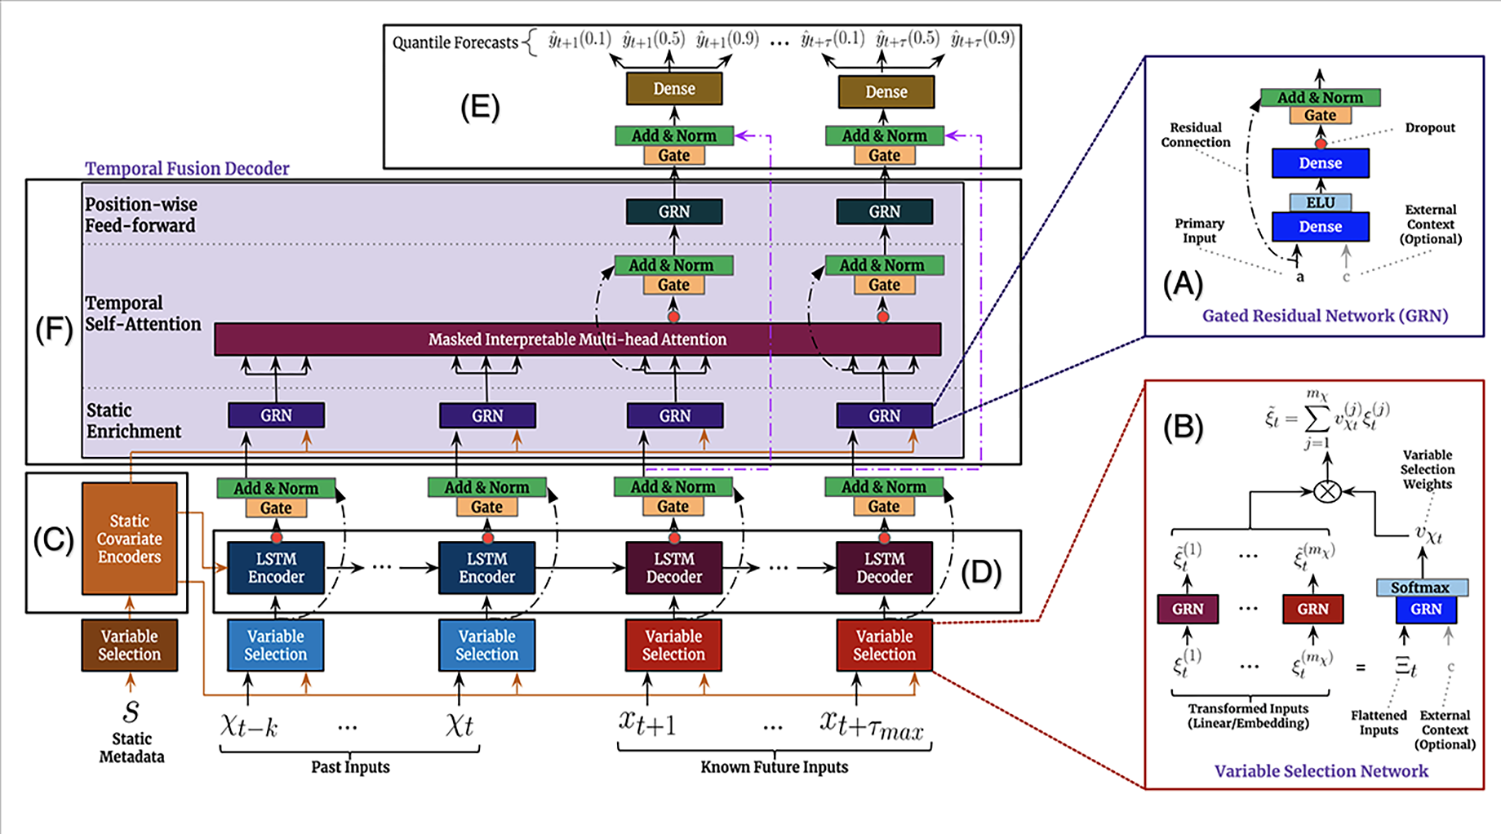
\includegraphics[width=0.98\columnwidth]{figs/tft_architecture.png}}{\fbox{Missing figure: figs/tft_architecture.png}}
    \caption{TFT architecture showing how static metadata, observed historical inputs, and known future inputs enter the model through different pathways before fusion via multi-head attention.}
    \label{fig:tft_architecture}
\end{figure}

Hyperparameters for all models were selected based on the 2020 validation set (primarily tuning on the $h=21$ case) and are detailed in Appendix B. Notably, the TFT required careful tuning of learning rate and regularization strength due to its complexity, and simpler architectures like the RNNs were less prone to overfit given the data volume. TFT is trained with a multi-horizon head, whereas RNNs/tabular baselines are trained separately per horizon; we favor realism in how these models are typically used over identical objective forms.

\section{Results}

Table~\ref{tab:main_results} summarizes performance across horizons. All $R^2$ values are near zero or slightly negative, reflecting the difficulty of short-horizon stock return prediction relative to a zero-return baseline. Nonetheless, RMSE and DA highlight consistent differences across model classes. 

At $h=1$, the LSTM attains the lowest RMSE (0.01622), narrowly outperforming GRU (0.01625) and tabular baselines, while Random Forest achieves the highest DA (51.9\%). At $h=5$, Ridge regression clearly dominates on RMSE (0.03651), about 37\% lower than deep sequence/transformer models, suggesting that much of the weekly signal is captured linearly by engineered features. At $h=21$, LSTM yields both the lowest RMSE (0.05084) and highest DA (55.0\%), within 0.03--0.24\% RMSE of GRU/TFT but 31--38\% lower than tabular baselines. Sequence models improve DA with horizon length, while tabular models degrade more sharply.

\begin{figure}[t]
    \centering
    % Include figure if available; otherwise show a placeholder to avoid compilation errors.
    \IfFileExists{../comparison/artifacts/figures/fig1_da_by_horizon.png}{\includegraphics[width=0.98\columnwidth]{../comparison/artifacts/figures/fig1_da_by_horizon.png}}{\fbox{Missing figure: fig1_da_by_horizon.png}}
    \caption{Directional accuracy by model and horizon on the test set (setup in Abstract). Sequence models (LSTM/GRU) particularly gain an edge at $h{=}21$.}
    \label{fig:da_by_horizon}
\end{figure}

% (Equity curve figure removed; strategy diagnostics not part of this study's evaluation.)

\begin{table*}[t]
    \centering
    \caption{Main results on the test set (setup in Abstract). Each cell shows mean $\pm$ std over 3 random seeds unless otherwise noted. \rTwo{} is calculated against a zero-return baseline. Metrics computed from our aggregated results file (\texttt{Table1\_EXP-A.csv}).}
    \label{tab:main_results}
    \sisetup{round-mode=places,round-precision=6}
    \begin{tabular}{llccc}
        \toprule
        Model & Horizon $h$ & $\rmse$ & $\rTwo$ & $\da$ \\
        \midrule
        GRU            & 1  & 0.016249 $\pm$ 0.000047 & -0.006072 & 0.500920 $\pm$ 0.024931 \\
        GRU            & 5  & 0.057883 $\pm$ 0.000123 & -0.002885 & 0.542105 $\pm$ 0.036308 \\
        GRU            & 21 & 0.050854 $\pm$ 0.000059 & -0.002185 & 0.539142 $\pm$ 0.033861 \\
        LSTM           & 1  & \textbf{0.016222} $\pm$ 0.000025 & -0.002677 & 0.516688 $\pm$ 0.015768 \\
    LSTM           & 5  & 0.057849 $\pm$ 0.000048 & -0.001694 & \textbf{0.554207} \\
    LSTM           & 21 & \textbf{0.050840} $\pm$ 0.000070 & -0.001629 & \textbf{0.550429} \\
        Random Forest  & 1  & 0.016387 $\pm$ 0.000007 & -0.023148 & \textbf{0.519454} $\pm$ 0.000290 \\
        Random Forest  & 5  & 0.039717 $\pm$ 0.000175 & -0.206505 & 0.531379 $\pm$ 0.000636 \\
        Random Forest  & 21 & 0.081805 $\pm$ 0.000151 & -0.248432 & 0.542956 $\pm$ 0.001095 \\
    Ridge          & 1  & 0.016346 & -0.018058 & 0.500254 \\
    Ridge          & 5  & \textbf{0.036514} & -0.019737 & 0.511699 \\
    Ridge          & 21 & 0.074214 & -0.027501 & 0.528230 \\
        TFT            & 1  & 0.016453 $\pm$ 0.000313 & -0.031783 & 0.489379 $\pm$ 0.019597 \\
        TFT            & 5  & 0.057907 $\pm$ 0.000108 & -0.003690 & 0.550134 $\pm$ 0.012030 \\
        TFT            & 21 & 0.050963 $\pm$ 0.000225 & -0.006502 & 0.538742 $\pm$ 0.029354 \\
    XGBoost        & 1  & 0.016464 & -0.032850 & 0.515368 \\
    XGBoost        & 5  & 0.038217 & -0.117070 & 0.508611 \\
    XGBoost        & 21 & 0.081344 & -0.234415 & 0.516713 \\
        \bottomrule
    \end{tabular}
    
    \vspace{0.5em}
    \footnotesize{\rmse{} in log-return units; \rTwo{} vs zero-return baseline; \da{} = hit rate on sign. Entries without $\pm$ denote single run; no variance.}
\end{table*}

Ridge's win at $h=5$ suggests much of the weekly signal is approximately linear in our engineered features.

\subsection{Hypothesis Evaluation}

	\textbf{H1 (Model class advantage):} Not supported. At $h=21$, TFT does not outperform the strongest non-TFT model. LSTM achieves the lowest RMSE (0.05084 vs.\ TFT's 0.05096, a 0.24\% edge) and the highest DA (55.0\% vs.\ TFT's 53.9\%, +1.1 pp). Standard deviations overlap, and the differences do not meet our decision thresholds ($\geq$2 pp DA or $\geq$5\% RMSE). Formal Diebold--Mariano and McNemar tests confirm no statistically significant advantage for TFT ($p > 0.05$). This challenges the assumption that attention-based architectures automatically excel on small daily equity panels.

    	\textbf{H2 (Event features add value):} Supported. Ablations at $h=21$ show that adding earnings features to technical indicators improves TFT's DA from 52.2\% to 53.3\% (+1.1 pp) while slightly reducing RMSE (0.05128 $\rightarrow$ 0.05094). More strikingly, during $\pm 3$ day earnings windows, DA rises to 61.4\% compared to 53.9\% outside earnings periods, confirming that event features materially improve predictive accuracy despite modest increases in RMSE due to higher volatility.

	\textbf{H3 (Regime dependence):} Supported. Model rankings shift markedly across regimes at $h=21$. In the 2022 bear market, GRU achieves the lowest RMSE (0.0636), but all models fall below 50\% DA. In contrast, during the 2023--2024 rally, LSTM achieves the lowest RMSE (0.0475) and both LSTM/GRU reach DA of 56.2\%, demonstrating strong directional performance in trending upward markets. These results align with the Adaptive Markets Hypothesis: sequence models thrive in rally regimes but fail to sustain accuracy in high-volatility downturns.

% Figure removed: replaced by Table~\ref{tab:main} presenting the full metrics.

\subsection{Ablations at h=21}
To understand the contribution of different feature types, we conducted an ablation study at the 21-day horizon. \Cref{tab:ablation} reports results (mean $\pm$ std over seeds) for experiments using: technical indicators only (B1) vs. technical+earnings features (B2). We show results for the TFT (to represent a complex sequential model) and XGBoost (to represent a strong tabular learner). Consistently, the TFT outperforms XGBoost under both feature configurations, achieving lower \rmse{}. Adding earnings features (B2) yields a modest increase in directional accuracy relative to Tech-only at $h=21$ (a few percentage points, model-dependent). Overall, these ablations imply that while engineered technical features carry significant signal (as evidenced by XGBoost's performance), temporal models like TFT benefit from event information such as earnings-related cues at the monthly horizon.

\begin{table}[t]
    \centering
    \caption{Ablations at $h=21$ (test). B1: technical only; B2: technical+earnings. Mean $\pm$ std over seeds; entries without $\pm$ denote single run.}
    \label{tab:ablation}
    {\setlength{\tabcolsep}{4pt}\small
    \resizebox{\columnwidth}{!}{%
    \begin{tabular}{llccc}
        \toprule
        Exp & Model & $\rmse$ & $\rTwo$ & $\da$ \\
        \midrule
    B1 & TFT      & 0.051284 $\pm$ 0.000748 & -0.019333 & 0.522187 $\pm$ 0.048917 \\
    B1 & XGBoost  & 0.081709 & -0.245491 & 0.511481 \\
    B2 & TFT      & \textbf{0.050936} $\pm$ 0.000112 & -0.005411 & \textbf{0.533232} $\pm$ 0.027920 \\
    B2 & XGBoost  & 0.081235 & -0.231083 & 0.517730 \\
        \bottomrule
    \end{tabular}}}
\end{table}

% Figure removed: ablation summary is now reported solely in Table~\ref{tab:ablation}.

\subsection{Regime and Earnings Slices (h=21)}
We evaluate performance by market period and around earnings.

    	\textbf{Market periods.} \Cref{fig:regime_heatmap} shows test \rmse{} split into the 2022 bear market and the 2023--24 rally. In 2022, errors rise for all models; GRU has the lowest \rmse{} (0.0636), yet the best \da{} (TFT, 48.08\%) is still below 50\%, indicating direction was hard to predict during the sell-off. In 2023--24, errors fall and \da{} improves: LSTM has the lowest \rmse{} (0.0475) and, with GRU, the highest \da{} ($\approx 56.23\%$). Sequence models appear to benefit from the upward trend (Table~\ref{tab:regimes}).

\textbf{Earnings windows.} As shown in Table~\ref{tab:earnings}, average \da{} within \(\pm3\) days of earnings is 0.6136 (61.4\%) vs.\ 0.5386 (53.9\%) outside, while \rmse{} is slightly higher during earnings (0.0695 vs.\ 0.0665), consistent with larger price moves. The improvement likely reflects informative earnings-surprise signals (positive surprises often precede up moves; negative surprises, down moves).

Overall, models are sensitive to both market period (sequence models thrive in rallies) and event timing (higher accuracy around earnings).


\begin{figure}[t]
    \centering
    % Include figure if available; otherwise show a placeholder to avoid compilation errors.
    \IfFileExists{../comparison/artifacts/figures/fig2_regime_rmse_heatmap.png}{\includegraphics[width=0.98\columnwidth]{../comparison/artifacts/figures/fig2_regime_rmse_heatmap.png}}{\fbox{Missing figure: fig2_regime_rmse_heatmap.png}}
    \caption{Test \rmse{} by model in two distinct market regimes: the 2022 bear market (left) and the 2023--24 rally (right). Darker shading indicates lower error. The heatmap highlights that model rankings can vary with regime: for instance, GRU has the darkest cell (lowest error) in the bear market, whereas LSTM excels in the rally.}
    \label{fig:regime_heatmap}
\end{figure}

\begin{table}[t]
    \centering
    \caption{Best models by regime at $h=21$ (test).}
    \label{tab:regimes}
    {\setlength{\tabcolsep}{4pt}\small
    \resizebox{\columnwidth}{!}{%
    \begin{tabular}{l l c l c}
        \toprule
        Regime & Best-$\rmse$ & $\rmse$ & Best-$\da$ & $\da$ \\
        \midrule
        Bear 2022       & GRU  & 0.0636 & TFT            & 0.4808 \\
        Rally 2023--24  & LSTM & 0.0475 & GRU/LSTM (tie) & 0.5623 \\
        \bottomrule
    \end{tabular}}}
\end{table}

\begin{table}[t]
    \centering
    \caption{Performance during earnings announcement windows vs. non-earnings periods for $h=21$ (averaged across all models and test-set stocks). During the $\pm3$ day earnings windows, directional accuracy (\da{}) is markedly higher, albeit with slightly higher \rmse{} due to greater volatility.}
    \label{tab:earnings}
    \begin{tabular}{lcc}
        \toprule
        Slice & $\rmse$ & $\da$ \\
        \midrule
        Earnings window ($\pm3$ days) & 0.06951 & 0.61355 \\
        Non-earnings periods         & 0.06655 & 0.53860 \\
        \bottomrule
    \end{tabular}
\end{table}

\paragraph{Interpretation} These analyses indicate that simple sequence models (LSTM/GRU) are highly competitive for capturing directional moves, especially in more predictable regimes or longer horizons, whereas complex architectures like TFT may require more data or richer features to shine. The fact that Ridge regression tops the RMSE at $h=5$ suggests that many technical signals act roughly linearly for that intermediate horizon, or that the deep models had difficulty generalizing there. Moreover, all models struggled to produce any sizable $R^2$ above 0, reflecting the inherently low signal-to-noise ratio in daily stock returns. Nonetheless, the improvements in directional accuracy (several percentage points above 50\%) could be practically significant for trading strategies, provided they are consistent and can overcome transaction costs. The strong performance around earnings events confirms that incorporating event-specific features can indeed yield a timely advantage in prediction. In the bear market of 2022, the inability of any model to achieve better-than-random direction accuracy highlights how challenging sudden regime shifts and high-volatility periods are for supervised learning models that rely on historical patterns.

\section{Discussion}

\subsection{Hypothesis Implications}

Our hypothesis-driven evaluation yields three main insights on transformer efficacy in financial time series. First, H1 (TFT superiority) is rejected: on a constrained daily panel with technical and earnings features, attention mechanisms do not automatically improve prediction. LSTM's edge at \(h=21\) (over TFT) likely reflects a simpler inductive bias better matched to the low signal-to-noise ratio in daily returns.

Second, H2 (event features) holds, but timing matters. The ablation shows modest gains (+1.1\,pp \da{} for TFT), whereas leveraging explicit earnings windows drives a larger effect (+7.5\,pp \da{}; 61.4\% vs.\ 53.9\%), indicating that concentrating signal around events beats diluting it across all days (with a slight RMSE trade-off: 0.0695 vs.\ 0.0666).

Third, H3 (regime dependence) is confirmed: no single model dominates across markets. Sequence models (LSTM/GRU) excel in rallies but falter in bears; \da{} dipped below 50\% in 2022, suggesting supervised models trained on historical patterns can struggle under acute stress. This favors ensembles or regime-switching approaches.

Overall, at daily frequency and a small universe, simpler models can match or beat more complex ones. LSTM/GRU (fewer parameters) rival TFT here---excess capacity can hinder training or overfit sparse signals. Tabular methods remain strong: Ridge attains the lowest \rmse{} at \(h=5\), implying a regularized linear mix of technicals captures much of the limited weekly predictability, while deep models better capture directional patterns (e.g., trend persistence) at \(h=21\).

All models leave most variance unexplained (\rTwo{}\(\approx 0\)), which is consistent with efficient-market arguments. Small edges still matter: \(\sim\)55\% \da{} at \(h=21\) (LSTM) could be economically meaningful if paired with a trading strategy---outside our scope---but only if it generalizes, hence our strict temporal holdout.

\textit{Practical guidance.} (i) For very short horizons (daily), start with linear or tree models plus well-chosen features; complex sequence models may not help. (ii) For monthly horizons, RNNs (LSTM) better capture directional swings. (iii) Transformers (e.g., TFT) are more promising with richer covariates or larger cross-sections (their comparative advantage is multimodal fusion and long-range dependencies).


\textbf{Limitations and threats to validity.} Scope is limited to the Dow 30 and daily data; we did not include unstructured/alternative modalities or test cross-universe generalization. Despite temporal splits and purging, overlapping multi-horizon targets introduce dependence. Our tuning budget was modest, which can favor simpler models. Comparing single-horizon tabular/RNN models to multi-horizon TFT raises fairness concerns; we trained separate single-horizon variants where feasible and note residual differences. Future work includes richer covariates (e.g., sentiment, macro), alternative objectives (e.g., quantile loss), reinforcement-learning policies, and interpretability analyses (e.g., TFT attention, SHAP) to clarify drivers across regimes.


\section{Conclusion}
We benchmarked transformer, recurrent, and traditional models for multi-horizon stock return prediction on the Dow 30 using technical and earnings features under a strict time split. Findings are: (H1) on this daily, data-constrained panel, transformers did not dominate---LSTM performed best at the 21-day horizon (lowest \rmse{}, highest \da{}); (H2) earnings/event features add value, especially within \(\pm\)3-day earnings windows (+7.5\,pp \da{}); and (H3) model rankings are regime-dependent---sequence models fare better in bullish trends and struggle in bear markets.

Across horizons, Ridge achieved the best 5-day \rmse{}, and Random Forest led 1-day \da{}. Thus, well-tuned simpler models can rival or surpass more complex ones in this setting. This negative result for (H1) tempers assumptions about architectural complexity without ruling out transformer gains on larger universes or with richer covariates.

We offer these results as a baseline: future work should compare against these controls under similar splits and features, and test whether alternative data or higher-frequency signals allow architectures like TFT to exceed where simpler models plateau.


\subsection*{Future Work}
We plan to extend this comparison along several dimensions: (i) add alternative data modalities (e.g., textual sentiment or macro indicators) to test multi-modal fusion; (ii) broaden the universe (e.g., S\&P 100 or global equities) and add rolling-origin evaluations; (iii) explore objective functions beyond MSE (e.g., quantile or asymmetric losses) and cost-aware metrics; and (iv) investigate regime-aware ensembling and calibration. Integrating news-derived or event-text signals is a natural next step, but it is outside the scope of the present experiments.


% Use IEEEtran's natbib-compatible style to support \citet/\citep
{\small
\bibliographystyle{IEEEtranN}
\bibliography{references}
}

% \appendix
% \section*{Appendix A: Dow 30 Constituents (frozen as of 2018-01-01)}
% \begin{small}
% \begin{tabular}{ll}
% \toprule
% Ticker & Company \\
% \midrule
% AAPL & Apple Inc. \\
% AXP & American Express Co. \\
% BA & Boeing Co. \\
% CAT & Caterpillar Inc. \\
% CSCO & Cisco Systems, Inc. \\
% CVX & Chevron Corporation \\
% DIS & Walt Disney Company \\
% DWDP & DowDuPont Inc. \\
% GE & General Electric Co. \\
% GS & Goldman Sachs Group, Inc. \\
% HD & Home Depot, Inc. \\
% IBM & Int'l Business Machines Corp. \\
% INTC & Intel Corporation \\
% JNJ & Johnson \& Johnson \\
% JPM & JPMorgan Chase \& Co. \\
% KO & Coca-Cola Company \\
% MCD & McDonald's Corporation \\
% MMM & 3M Company \\
% MRK & Merck \& Co., Inc. \\
% MSFT & Microsoft Corporation \\
% NKE & NIKE, Inc. \\
% PFE & Pfizer Inc. \\
% PG & Procter \& Gamble Co. \\
% TRV & Travelers Companies, Inc. \\
% UNH & UnitedHealth Group Inc. \\
% UTX & United Technologies Corp. \\
% V   & Visa Inc. \\
% VZ  & Verizon Communications Inc. \\
% WMT & Walmart Inc. \\
% XOM & Exxon Mobil Corporation \\
% \bottomrule
% \end{tabular}
% \end{small}

% \section*{Appendix B: Training Details and Hyperparameters}
% \begin{small}
% \begin{itemize}
%     \item \textbf{Training procedure:} After tuning on Val-2020, all models are refit on Train$+$Val. Neural nets use Adam/AdamW up to 10 epochs with early stopping on a held-out contiguous slice within 2020 (forward-only). GRU/LSTM use base learning rate $1\times10^{-3}$; TFT uses $3\times10^{-4}$. Batch size 256. Final metrics computed once on Test (2021--2024).
%     \item \textbf{RNNs:} 1 layer GRU/LSTM with 64 hidden units (tuned on val). Dropout 0.2 on input sequences. Lookback window = 60 days.
%     \item \textbf{TFT:} 4 attention heads, 1 transformer layer, hidden dimensionality 16 in fully connected layers, dropout 0.3. Trained to predict all 3 horizons jointly. Total parameters $\approx$50k.
%     \item \textbf{Random Forest:} 100 trees, max depth 5 (to prevent overfitting), other parameters default.
%     \item \textbf{XGBoost:} max depth 3, learning rate 0.1, 100 boosting rounds. (Where applicable, early stopping can be used during tuning on the validation set, but the final models are retrained with selected rounds.)
%     \item \textbf{Ridge:} Regularization $\alpha$ tuned via cross-val on train set, ended around $\alpha \approx 1.0$.
%     \item \textbf{Standardization:} Features standardized (zero mean, unit std) per feature across train data. The same scaler parameters are applied to val/test.
%         \item \textbf{Hyperparameter selection and tuning protocol (all models):} We performed lightweight tuning exclusively on the contiguous Val-2020 block to avoid look-ahead. For tabular models we used small grid/random sweeps with the selection objective set to RMSE at $h{=}21$ (primary horizon), then fixed hyperparameters across horizons for fairness and to reduce variance. For neural models we tuned core capacity and regularization parameters and relied on early stopping for epoch selection. Seeds $\{42,43,44\}$ were kept fixed across candidates to reduce selection noise.
%         \begin{itemize}
%             \item \emph{Ridge:} $\alpha\in\{10^{-3},10^{-2},10^{-1},1,10,10^{2},10^{3}\}$; choose by Val-2020 RMSE.
%             \item \emph{Random Forest:} $n$\,estimators $\in\{100,300\}$, max\_depth $\in\{\texttt{None},5,7\}$, min\_samples\_leaf $\in\{1,5,10\}$; we constrained depth to mitigate overfitting on a small daily panel.
%             \item \emph{XGBoost:} max\_depth $\in\{3,4,5\}$, learning rate $\in\{0.05,0.1\}$, subsample/colsample\_bytree $\in\{0.7,1.0\}$; number of rounds selected via early stopping on Val-2020, then refit.
%             \item \emph{GRU/LSTM:} hidden units $\in\{32,64,128\}$, dropout $\in\{0.1,0.2,0.3\}$, learning rate $\in\{5\times10^{-4},1\times10^{-3}\}$, weight decay $\in\{0,10^{-5},10^{-4}\}$; 1 layer favored for bias/variance balance.
%             \item \emph{TFT:} attention heads $\in\{2,4\}$, transformer layers $\in\{1,2\}$, hidden size $\in\{16,32\}$, dropout $\in\{0.2,0.3,0.4\}$, learning rate $\in\{3\times10^{-4},1\times10^{-3}\}$. We intentionally kept capacity modest given dataset size and absence of rich exogenous covariates.
%         \end{itemize}
%         \item \textbf{Defaults vs. tuned choices:} We validated that common library defaults are ill-suited for this setting: e.g., Random Forest with unlimited depth or XGBoost with deeper trees and higher learning rate tended to overfit Val-2020 and degrade on Test; we therefore used shallow trees and lower learning rates. Ridge defaults ($\alpha{=}1$) were close to tuned picks and served as a strong baseline. For deep models, larger hidden sizes ($\geq$128) and deeper TFT stacks increased variance without improving validation error, hence the smaller-capacity selections. We focused the paper on tuned models for a fair, competence-bound comparison; default-only results are not included in the main tables to conserve space but can be reproduced by disabling the tuning grid and using library defaults in our training scripts.
% \end{itemize}
% \end{small}


\end{document}

